\begin{comment}
\end{comment}

\chapter{Résultats}

%-----------------------------------------------------------------------------%

\section{Exemple de graphique}

La figure~\ref{fig:phdcomics} est très drôle, sérieusement.

\begin{figure}[htb]
    \begin{center}
        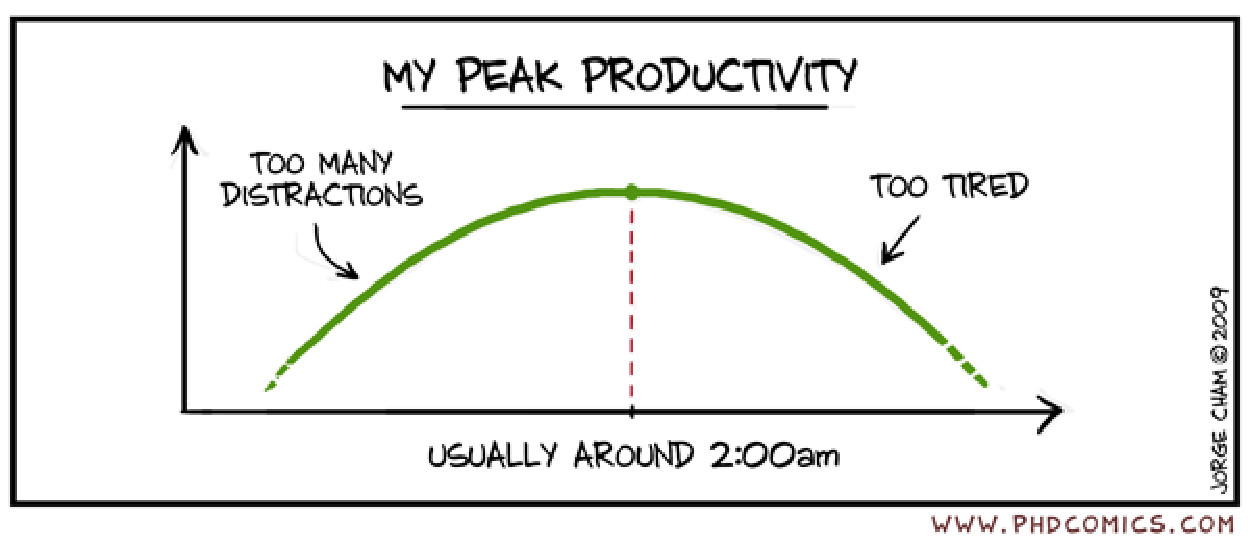
\includegraphics[width=0.8\columnwidth]{figures/phd083109s.pdf} 
        \longcaption{Figure à la fois hilarante et véridique.}{Image tirée du webcomic "Piled Higher and Deeper" par Jorge Cham \href{www.phdcomics.com}{www.phdcomics.com}. Seule la première partie de ce long caption sera dans la table des figures.}
        \label{fig:phdcomics}
    \end{center}
\end{figure}

\section{Remplissage}
\kant[11-14]
